\chapter{Light Cones, Geodesics, and the Schwarzschild Horizon}

The horizon problem begins with a distinction already present in special
relativity.  Two nearby events may be separated in a time-like, space-like, or
light-like direction.  Curvature does not abolish this classification.  It
makes the light cone a local object, different at every event, and makes the
metric itself dynamical.  Once the metric is known, the motion of a freely
falling particle follows from the same proper-time principle that describes a
free relativistic particle in flat spacetime.

We shall use that principle twice.  First it must reproduce Newtonian motion in
a weak field.  Then it will be applied to the Schwarzschild metric, where the
meaning of time, radial distance, and velocity becomes unexpectedly subtle.

\section{Time-like, Space-like, and Light-like Intervals}

In flat spacetime, with \(c=1\), the proper-time element is
\begin{equation}
d\tau^2=dt^2-dx^2-dy^2-dz^2.
\label{eq:l5-minkowski-proper-time}
\end{equation}
Restoring \(c\) is useful whenever a nonrelativistic approximation is near:
\begin{equation}
d\tau^2
=dt^2-\frac{dx^2+dy^2+dz^2}{c^2}.
\label{eq:l5-minkowski-c}
\end{equation}
The notation \(d\tau^2\) does not guarantee that the right-hand side is
positive.  Its sign classifies the displacement:
\begin{align}
d\tau^2>0
&\quad\Longleftrightarrow\quad \text{time-like},\\
d\tau^2=0
&\quad\Longleftrightarrow\quad \text{light-like},\\
d\tau^2<0
&\quad\Longleftrightarrow\quad \text{space-like}.
\end{align}
For a space-like displacement it is convenient to define the positive proper
distance
\begin{equation}
ds^2=-d\tau^2
=dx^2+dy^2+dz^2-dt^2
\qquad(c=1).
\label{eq:l5-proper-distance}
\end{equation}

The light cone organizes these three possibilities.  Its surface, not its
filled interior, consists of the light-like directions.  Time-like directions
lie inside the cone and space-like directions lie outside.  The upper and
lower halves represent the future and past light cones.

\begin{figure}[htbp]
\centering

\includegraphics[width=0.82\textwidth]{lecture_05_figure_02.png}
\caption{Proper time, proper distance, and the causal cone assembled on the
board.  Light rays occupy the cone itself; the interior is time-like and the
exterior is space-like.}
\lectureframe{00:05:44}
\end{figure}

\begin{figure}[htbp]
\centering
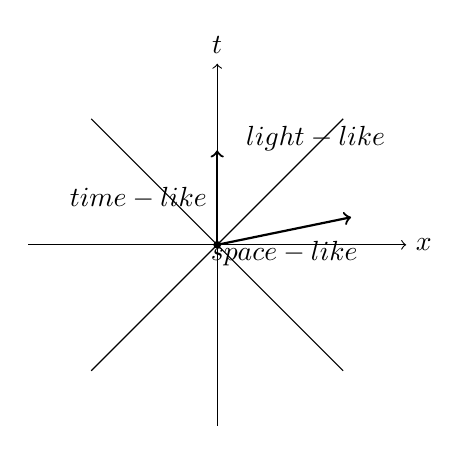
\begin{tikzpicture}[scale=1.0]
\draw[->] (0,-2.3) -- (0,2.3) node[above] {\(t\)};
\draw[->] (-2.4,0) -- (2.4,0) node[right] {\(x\)};
\draw (-1.6,1.6) -- (0,0) -- (1.6,1.6);
\draw (-1.6,-1.6) -- (0,0) -- (1.6,-1.6);
\fill (0,0) circle (1.4pt);
\draw[->,thick] (0,0) -- (0,1.2)
  node[midway,left] {\(\text{time-like}\)};
\draw[->,thick] (0,0) -- (1.7,0.35)
  node[midway,below] {\(\text{space-like}\)};
\node at (1.25,1.35) {\(\text{light-like}\)};
\end{tikzpicture}
\caption{The causal classification in a two-dimensional spacetime section.}
\end{figure}

These intervals are operational.  Proper time is what a clock carried along a
time-like worldline reads.  Proper distance is what a suitable set of meter
sticks measures between space-like separated events.  They are not merely
names for signs in a quadratic form.

\section{Lorentzian Signature and a Cone at Every Event}

Using the mostly-plus tensor convention, the flat metric has components
\begin{equation}
\eta_{\mu\nu}=\operatorname{diag}(-1,1,1,1),
\label{eq:l5-eta}
\end{equation}
and
\begin{equation}
d\tau^2=-\eta_{\mu\nu}\,dx^\mu dx^\nu.
\label{eq:l5-proper-time-eta}
\end{equation}
The displayed matrix is the expression of a rank-two tensor in one especially
simple basis.  Its invariant feature is its signature: one negative and three
positive directions,
\begin{equation}
\operatorname{signature}(\eta)=(-,+,+,+).
\label{eq:l5-lorentz-signature}
\end{equation}
A metric with two negative signs would have two temporal directions.  Such
signatures can be studied mathematically, but they do not describe the
spacetime assumed here.

In curved spacetime the components vary:
\begin{equation}
g_{\mu\nu}=g_{\mu\nu}(x).
\label{eq:l5-position-metric}
\end{equation}
At each event the metric must still have Lorentzian signature.  Consequently,
each event has its own time-like directions, light-like boundary, and
space-like directions.  A coordinate drawing may show cones tilted or
squashed from point to point, but the causal classification remains.

\begin{figure}[htbp]
\centering

\includegraphics[width=0.86\textwidth]{lecture_05_figure_03.png}
\caption{The position-dependent metric \(g_{\mu\nu}(x)\), the causal labels,
and sketches of local light cones.}
\lectureframe{00:09:41}
\end{figure}

\begin{figure}[htbp]
\centering
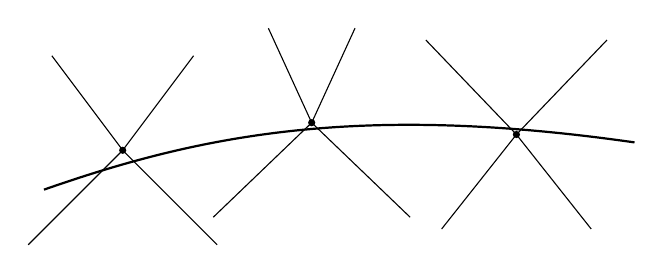
\begin{tikzpicture}[scale=1.0]
\draw[thick] (-4,-0.5) .. controls (-2,0.2) and (0,0.6) .. (3.5,0.1);
\foreach \x/\y/\a/\b in {-3/0/0.9/1.2, -0.6/0.35/0.55/1.25,
                          2.0/0.2/1.15/0.95} {
  \fill (\x,\y) circle (1.3pt);
  \draw (\x,\y) -- ++(-\a,1.2);
  \draw (\x,\y) -- ++(\a,1.2);
  \draw (\x,\y) -- ++(-\b,-1.2);
  \draw (\x,\y) -- ++(\b,-1.2);
}
\end{tikzpicture}
\caption{Neighboring local cones.  Their coordinate shape can change without
changing which vectors are time-like, light-like, or space-like.}
\end{figure}

\begin{classroomqa}
\audiencequestion{Does the single negative eigenvalue select one unique
time direction?}
\lecturerresponse{A basis that diagonalizes the displayed matrix has one
negative basis direction, but that does not select a preferred observer or a
unique physical arrow.  Lorentz transformations mix the time coordinate with
space coordinates, and every vector inside the cone is time-like.  The
invariant object is the cone together with the one-minus, three-plus
signature, not one distinguished time-like vector.
\lecturetimestamp{00:12:17--00:17:24}}
\end{classroomqa}

\begin{classroomqa}
\audiencequestion{Why can two drawings of the local cone have different
shapes?}
\lecturerresponse{Coordinates can change the drawing.  For example, replacing
\(x\) by a rescaled coordinate changes the numerical slope assigned to a light
ray and therefore makes the cone appear narrower or wider.  More general
coordinates can tilt it.  The same event and the same causal relations are
being represented.  In curved spacetime cones at distinct events also belong
to distinct tangent spaces, so their comparison requires the metric and a
transport rule.
\lecturetimestamp{00:13:37--00:15:59}}
\end{classroomqa}

\section{Geodesics as a Variational Problem}

A freely moving particle follows a spacetime geodesic.  In differential form,
using an affine parameter \(\lambda\),
\begin{equation}
\frac{d^2x^\mu}{d\lambda^2}
+\Gamma^\mu{}_{\rho\sigma}
\frac{dx^\rho}{d\lambda}
\frac{dx^\sigma}{d\lambda}=0.
\label{eq:l5-geodesic}
\end{equation}
The connection tells the tangent how to remain parallel to itself as the
particle moves.

There is a second formulation that is often easier to calculate with.  In a
Riemannian space with metric \(g_{mn}\), the length of a curve is
\begin{equation}
s=\int ds
=\int\sqrt{g_{mn}\,dx^m dx^n}.
\label{eq:l5-spatial-length}
\end{equation}
The geodesic makes this length stationary under small variations of the path
with fixed endpoints.  The integral is simply the sum of infinitesimal lengths
along the curve, and its Euler--Lagrange equation is a second-order
differential equation analogous in form to a force law.

For a time-like worldline, spatial length is replaced by proper time:
\begin{equation}
\tau
=\int\sqrt{-g_{\mu\nu}\,dx^\mu dx^\nu}.
\label{eq:l5-proper-time-functional}
\end{equation}
A time-like geodesic makes \(\tau\) stationary and, for nearby freely falling
paths before conjugate points occur, locally maximal.  Multiplying by
\(-m\) gives the particle action
\begin{equation}
A=-m\tau
=-m\int\sqrt{-g_{\mu\nu}\,dx^\mu dx^\nu}.
\label{eq:l5-particle-action}
\end{equation}
Thus the same path locally minimizes \(A=-m\tau\).  The distinction between a
stationary proper time and the sign of the chosen action removes the apparent
minimum-versus-maximum ambiguity.

\section{From Proper Time to an Ordinary Lagrangian}

The action in \eqref{eq:l5-particle-action} is geometric, but it can be put in
the familiar form used in mechanics.  Parameterize the worldline by the
coordinate \(t\), divide each differential by \(dt\), and pull the remaining
factor of \(dt\) outside the square root:
\begin{align}
A
&=-m\int\sqrt{-g_{\mu\nu}(x)\,dx^\mu dx^\nu}\\
&=-m\int
\sqrt{-g_{\mu\nu}(x)
\frac{dx^\mu}{dt}\frac{dx^\nu}{dt}}\,dt.
\label{eq:l5-action-t}
\end{align}
For the temporal component \(dt/dt=1\); the spatial components are ordinary
coordinate velocities.  We may therefore write
\begin{equation}
A=\int L\,dt,
\qquad
L=-m\sqrt{-g_{\mu\nu}(x)\dot x^\mu\dot x^\nu},
\qquad
\dot x^\mu=\frac{dx^\mu}{dt}.
\label{eq:l5-relativistic-lagrangian}
\end{equation}

\begin{figure}[htbp]
\centering

\includegraphics[width=0.88\textwidth]{lecture_05_figure_05.png}
\caption{The worldline action being converted into the conventional form
\(A=\int L\,dt\).}
\lectureframe{00:27:00}
\end{figure}

\begin{figure}[htbp]
\centering

\includegraphics[width=0.88\textwidth]{lecture_05_figure_06.png}
\caption{A later board state with the relativistic Lagrangian isolated.}
\lectureframe{00:28:59}
\end{figure}

\begin{classroomqa}
\audiencequestion{Should the spacetime indices in this action be Greek?}
\lecturerresponse{Yes.  Greek indices run over time and all spatial
coordinates.  Latin indices may be reserved for the spatial coordinates when
that distinction is useful.
\lecturetimestamp{00:25:53--00:26:03}}
\end{classroomqa}

\begin{classroomqa}
\audiencequestion{Why is the square-root expression called the Lagrangian?}
\lecturerresponse{After the action has been written as \(A=\int L\,dt\), the
integrand is the Lagrangian.  This is not only a definition: varying that
integrand gives the Euler--Lagrange equations
\[
\frac{d}{dt}
\left(\frac{\partial L}{\partial\dot x^\mu}\right)
=\frac{\partial L}{\partial x^\mu},
\]
which are equivalent to the geodesic equation after the parameterization is
handled consistently.
\lecturetimestamp{00:28:36--00:29:02}}
\end{classroomqa}

For a massive particle the worldline is time-like, so the quantity under the
square root is positive.  A space-like path would describe superluminal
motion, not the trajectory of an ordinary massive particle.  Given a metric,
one can now obtain the particle's path either by computing the Christoffel
symbols and using \eqref{eq:l5-geodesic}, or by applying Euler--Lagrange to
\eqref{eq:l5-relativistic-lagrangian}.  Showing their equivalence is a useful
exercise; the action route is usually shorter.

\section{The Newtonian Limit}

Consider the weak, static gravitational field outside a spherical source.
Begin with flat spacetime and allow the coefficient of \(dt^2\) to differ
slightly from one:
\begin{equation}
d\tau^2
=\left(1+\frac{2u(\mathbf{x})}{c^2}\right)dt^2
-\frac{d\mathbf{x}^2}{c^2},
\label{eq:l5-weak-metric}
\end{equation}
where \(u\) is to become the Newtonian potential.  This ansatz must be checked,
not merely named.

The dimensionful particle action is
\begin{equation}
A=-mc^2\int
\sqrt{1+\frac{2u}{c^2}
-\frac{\dot{\mathbf{x}}^{\,2}}{c^2}}\,dt.
\label{eq:l5-weak-action}
\end{equation}
Both \(u/c^2\) and \(\dot{\mathbf{x}}^{\,2}/c^2\) are small.  Keeping their
first-order contributions,
\begin{equation}
\sqrt{1+\epsilon}
=1+\frac{\epsilon}{2}+O(\epsilon^2),
\qquad
\epsilon=\frac{2u-\dot{\mathbf{x}}^{\,2}}{c^2},
\end{equation}
gives
\begin{align}
L
&=-mc^2
\sqrt{1+\frac{2u-\dot{\mathbf{x}}^{\,2}}{c^2}}\\
&=-mc^2-mu+\frac{m}{2}\dot{\mathbf{x}}^{\,2}
+O(c^{-2}u^2,c^{-2}u\dot{\mathbf{x}}^{\,2},c^{-2}\dot{\mathbf{x}}^{\,4}).
\label{eq:l5-newton-expansion}
\end{align}
The constant rest-energy term has no effect on the equations of motion.  What
remains is
\begin{equation}
L_{\mathrm{nr}}
=\frac{m}{2}\dot{\mathbf{x}}^{\,2}-m u(\mathbf{x}),
\label{eq:l5-newton-lagrangian}
\end{equation}
and therefore
\begin{equation}
m\ddot{\mathbf{x}}=-m\boldsymbol{\nabla}u.
\label{eq:l5-newton-equation}
\end{equation}
The test mass cancels, as it must for universal free fall.  The potential
energy is \(m u\), while the acceleration is independent of \(m\).

We have consequently identified the leading weak-field relation
\begin{equation}
g_{00}=1+\frac{2u}{c^2}+O(c^{-4}).
\label{eq:l5-g00-newton}
\end{equation}
Outside a spherical mass \(M\),
\begin{equation}
u(r)=-\frac{GM}{r},
\qquad
g_{00}=1-\frac{2GM}{rc^2}+O(c^{-4}).
\label{eq:l5-g00-spherical}
\end{equation}
This determines the first correction to the time component.  It does not yet
determine the complete strong-field metric.

\section{Spherical Coordinates and the First Schwarzschild Guess}

Spherical coordinates are natural for a central source.  The lecture measures
\(\theta\) from the equatorial plane rather than from the pole, so its angular
line element is
\begin{equation}
d\Omega^2=d\theta^2+\cos^2\theta\,d\phi^2.
\label{eq:l5-angular-metric}
\end{equation}
With this convention,
\begin{equation}
d\mathbf{x}^2=dr^2+r^2d\Omega^2.
\label{eq:l5-flat-spherical}
\end{equation}
Nothing physical depends on choosing this latitude-like \(\theta\); using the
more common polar angle would replace \(\cos^2\theta\) by
\(\sin^2\theta\).

Inserting the Newtonian time coefficient while leaving the spatial metric
flat gives the first guess
\begin{equation}
d\tau^2
=\left(1-\frac{r_s}{r}\right)dt^2
-\frac{1}{c^2}\left(dr^2+r^2d\Omega^2\right),
\qquad
r_s=\frac{2GM}{c^2}.
\label{eq:l5-naive-schwarzschild}
\end{equation}
This cannot be the exact answer.  For \(r<r_s\), the coefficient of \(dt^2\)
changes sign while every spatial coefficient remains negative in the
proper-time convention.  The metric would lose its one-time, three-space
signature.

The vacuum field equations supply the required radial coefficient:
\begin{equation}
\boxed{
d\tau^2
=\left(1-\frac{r_s}{r}\right)dt^2
-\frac{dr^2}{c^2\left(1-r_s/r\right)}
-\frac{r^2}{c^2}d\Omega^2.
}
\label{eq:l5-schwarzschild}
\end{equation}
This is the exterior Schwarzschild metric.  When \(r\) passes through \(r_s\),
the \(t\) and \(r\) coefficients change sign together, preserving Lorentzian
signature.  In Schwarzschild coordinates the radial coordinate becomes
time-like inside and the coordinate \(t\) becomes space-like.  This exchange
signals a failure of the coordinate chart at the horizon, not a local failure
of the spacetime geometry.

\begin{classroomqa}
\audiencequestion{How long does a falling object take to cross the horizon?}
\lecturerresponse{Measured by the Schwarzschild coordinate \(t\) used by a
distant observer, the crossing is pushed to infinite time.  Measured by the
proper time on the falling object's clock, it occurs in finite time.  The
distinction between these clocks is the central horizon puzzle.
\lecturetimestamp{00:54:45--00:55:35}}
\end{classroomqa}

\begin{classroomqa}
\audiencequestion{Why alter the radial coefficient rather than some other
part of the metric?}
\lecturerresponse{The metric must retain Lorentzian signature, spherical
symmetry distinguishes the radial direction from the angular sphere, and the
vacuum field equations determine the reciprocal factor precisely.  Signature
alone motivates where to look; Einstein's equations give the exact result.
\lecturetimestamp{00:55:35--00:56:01}}
\end{classroomqa}

For the Earth, \(r_s\) is only of order a centimeter, deep inside the material
body.  The exterior vacuum metric is not valid there, so the Earth has no
Schwarzschild horizon.  An interior solution must replace it inside the
matter and match it at the surface.

\begin{classroomqa}
\audiencequestion{If \(t\) and \(r\) exchange coordinate roles, what happens
to an ordinary clock?}
\lecturerresponse{The clock continues to measure proper time along a
time-like worldline.  It does not know that a chosen coordinate has become
awkward.  A regular freely falling coordinate system shows smooth local
geometry and ordinary local light propagation through the horizon.
\lecturetimestamp{00:56:35--00:57:50}}
\end{classroomqa}

\subsection{Why the radial correction did not appear in Newton's equation}

The exact metric changes the radial coefficient already at first order in the
potential:
\begin{equation}
\frac{1}{1-r_s/r}
=1+\frac{r_s}{r}
+O\!\left(\frac{r_s^2}{r^2}\right)
=1-\frac{2u}{c^2}+O(c^{-4}).
\label{eq:l5-radial-expansion}
\end{equation}
Why was it legitimate to ignore that change in the Newtonian derivation?
Inside the particle action it multiplies \(\dot r^2/c^2\).  Its first
correction is therefore proportional to
\begin{equation}
\frac{u\,\dot r^2}{c^4},
\end{equation}
which is beyond the order retained in
\eqref{eq:l5-newton-expansion}.  The radial correction is negligible for the
slow-motion Newtonian test, yet it becomes decisive for relativistic motion
and near the horizon.  This is a useful warning: a term too small for one
approximation may control the phenomenon of interest in another.

\section{Radial Fall in Schwarzschild Time}

Set \(c=1\) and first study radial motion.  Circular orbits are also important,
but they require the angular terms and are postponed.  Radial motion is less
an orbit than a direct crash toward the source, and it exposes the horizon
behavior with the least algebra.

\begin{classroomqa}
\audiencequestion{Whose time appears in the radial velocity?}
\lecturerresponse{The dot below means differentiation with respect to the
Schwarzschild coordinate time \(t\), the time normalized to the distant
static observer.  The falling observer's wristwatch measures proper time
\(\tau\).  Confusing the two would turn a coordinate statement into a false
local one.
\lecturetimestamp{01:04:03--01:04:47}}
\end{classroomqa}

For \(d\Omega=0\), define
\begin{equation}
a(r)=1-\frac{r_s}{r}.
\label{eq:l5-a-def}
\end{equation}
The radial metric and Lagrangian are
\begin{align}
d\tau^2&=a\,dt^2-\frac{dr^2}{a},\\
L&=-m\sqrt{a-\frac{\dot r^2}{a}},
\qquad
\dot r=\frac{dr}{dt}.
\label{eq:l5-radial-lagrangian}
\end{align}
Because \(L\) has no explicit \(t\)-dependence, its Hamiltonian is conserved.
The radial momentum is
\begin{equation}
p_r=\frac{\partial L}{\partial\dot r}
=\frac{m\dot r}{a\sqrt{a-\dot r^2/a}},
\label{eq:l5-radial-momentum}
\end{equation}
and
\begin{align}
H
&=p_r\dot r-L\\
&=\frac{ma}{\sqrt{a-\dot r^2/a}}
=E.
\label{eq:l5-radial-energy}
\end{align}
Solving for the coordinate velocity gives
\begin{equation}
\boxed{
\dot r^2
=a^2\left(1-\frac{m^2}{E^2}a\right).
}
\label{eq:l5-radial-velocity}
\end{equation}
The board calculation tests several intermediate algebraic forms; the boxed
expression is the consistent result.

As \(r\) approaches \(r_s\), \(a(r)\) approaches zero while the factor in
parentheses approaches one.  Hence
\begin{equation}
\frac{dr}{dt}
\sim -\left(1-\frac{r_s}{r}\right)
\longrightarrow 0
\qquad(r\longrightarrow r_s^+)
\label{eq:l5-infall-freeze}
\end{equation}
for an ingoing particle.  In Schwarzschild time, the particle appears to slow
and freeze just outside the horizon.

\begin{classroomqa}
\audiencequestion{Does the decreasing value of \(dr/dt\) mean that gravity
has become repulsive?}
\lecturerresponse{No.  The particle is not locally pushed outward.  The
coordinate \(t\) becomes increasingly ill-suited to describing the crossing,
so radial progress per unit \(t\) tends to zero.  Proper acceleration along
the freely falling worldline remains zero, and the horizon is reached in
finite proper time.
\lecturetimestamp{01:14:18--01:16:38}}
\end{classroomqa}

Indeed, near the horizon
\begin{equation}
\frac{dt}{dr}
\sim-\frac{1}{1-r_s/r}
=-\frac{r}{r-r_s}.
\end{equation}
Its integral diverges logarithmically.  This proves the infinite
Schwarzschild-time statement without implying an infinite reading on the
falling clock.

\section{Radial Light Rays}

Light gives the shortest version of the same calculation.  For a radial null
ray,
\begin{equation}
d\tau^2
=a\,dt^2-\frac{dr^2}{a}=0.
\end{equation}
Therefore
\begin{equation}
\boxed{
\frac{dr}{dt}
=\pm a(r)
=\pm\left(1-\frac{r_s}{r}\right).
}
\label{eq:l5-radial-light}
\end{equation}
The plus sign describes an outgoing ray and the minus sign an ingoing ray.
Both coordinate speeds tend to zero at the horizon.

\begin{classroomqa}
\audiencequestion{What speed does the formula give far from the source?}
\lecturerresponse{As \(r\) tends to infinity, \(a(r)\) tends to one, so
\(dr/dt\) tends to \(\pm1\), or \(\pm c\) when units are restored.
\lecturetimestamp{01:21:01--01:21:29}}
\end{classroomqa}

General relativity is often like this: the principles fit in a few lines,
while coordinates and calculations grow complicated.  Equation
\eqref{eq:l5-radial-light} is simple, but interpreting its vanishing near
\(r_s\) requires care.  It is a coordinate speed, not the speed measured by a
local inertial observer.

\section{What a Distant Observer Sees}

\begin{classroomqa}
\audiencequestion{Can light emitted near the horizon escape, and is that
Hawking radiation?}
\lecturerresponse{An outgoing classical ray emitted just outside the horizon
can move outward, but its Schwarzschild coordinate speed begins extremely
small and the signal reaches infinity only after a severe delay and
redshift.  A ray on the horizon remains on the horizon in these coordinates;
a ray inside cannot escape.  Hawking radiation is a quantum-field effect
associated with the exterior geometry, not a classical light ray climbing
out from inside, and it is not derived by the present calculation.
\lecturetimestamp{01:22:08--01:24:28}}
\end{classroomqa}

\begin{classroomqa}
\audiencequestion{If a photon looks almost stationary, does it begin to look
massive?}
\lecturerresponse{No.  A freely falling local observer always measures the
photon moving at \(c\).  Only the coordinate ratio \(dr/dt\) tends to zero.
Mass, nullness, and the local speed of light are not changed by a bad
coordinate chart.
\lecturetimestamp{01:24:31--01:25:26}}
\end{classroomqa}

The Schwarzschild expression used here is a vacuum exterior solution.  A
star, planet, or collapsing cloud has a different interior metric that must
be matched to it.  If the material surface remains outside \(r_s\), as the
Earth's does by an enormous margin, the exterior coordinate horizon lies
outside the domain where the vacuum formula can be continued through the
matter.  If the body collapses inside its Schwarzschild radius, the horizon
becomes part of the physical spacetime.

\begin{classroomqa}
\audiencequestion{If an outside observer never sees matter cross, how can a
black hole ever form or grow?}
\lecturerresponse{The premise uses Schwarzschild time as though it were a
global physical clock at the horizon.  The conclusion that a black hole can
therefore never grow sounds plausible but is wrong.  A complete answer
requires regular horizon-crossing coordinates and the global causal geometry
of collapse; that resolution is deferred to the next stage of the course.
\lecturetimestamp{01:27:57--01:29:36}}
\end{classroomqa}

\begin{classroomqa}
\audiencequestion{What would a radar gun report for a car falling toward the
horizon?}
\lecturerresponse{The coordinate speed first increases as the car falls, then
turns over and decreases toward zero.  Radar pulses sent later can still catch
the car outside the horizon, but the round trip takes progressively longer.
The returned signal is increasingly redshifted, and the image appears slowed
and compressed near \(r_s\).  This is not a reliable local picture of what
the driver experiences; the driver crosses in finite proper time.
\lecturetimestamp{01:29:39--01:32:14}}
\end{classroomqa}

\begin{classroomqa}
\audiencequestion{Is the speed of light constant only in special
relativity?}
\lecturerresponse{It is constant in every local inertial frame in general
relativity as well.  An observer falling with local clocks and meter sticks
measures a nearby photon at \(c\).  Coordinate speeds such as \(dr/dt\) may
vary because \(r\) and \(t\) are not the readings of one local inertial
laboratory over the whole spacetime.
\lecturetimestamp{01:32:20--01:34:20}}
\end{classroomqa}

\section{Questions Beyond the Schwarzschild Calculation}

\begin{classroomqa}
\audiencequestion{What might it mean to unify gravity with the other
forces?}
\lecturerresponse{One geometric possibility is to enlarge spacetime with
additional compact directions.  Components of a higher-dimensional metric
can then appear in four dimensions as gauge fields and scalar fields, while
momentum in an extra direction can appear as a charge.  This is a structural
hint associated with Kaluza--Klein ideas, not a completed unification in the
present lecture.
\lecturetimestamp{01:34:22--01:36:08}}
\end{classroomqa}

\begin{classroomqa}
\audiencequestion{Could different regions or universes have different metric
signatures?}
\lecturerresponse{Classical general relativity ordinarily fixes a
nondegenerate Lorentzian signature.  Changing it would require the metric to
pass through a degenerate configuration, where the standard classical
description fails.  Quantum gravity may force a broader language, but there
is no established theory here that predicts physical signature-changing
regions.
\lecturetimestamp{01:36:08--01:38:08}}
\end{classroomqa}

\begin{classroomqa}
\audiencequestion{How did Schwarzschild find this solution while serving
during the First World War?}
\lecturerresponse{The point made in class is human as much as historical:
Schwarzschild was an astronomer and a highly accomplished mathematician, and
working through Einstein's new equations offered an intellectual refuge amid
wartime service.
\lecturetimestamp{01:38:11--01:39:02}}
\end{classroomqa}

The central lesson is now sharp enough to carry forward.  The metric
determines both causal cones and free motion.  Its weak-field time component
contains Newton's potential, while its exact Schwarzschild form gives a
coordinate horizon at \(r=r_s\).  Schwarzschild time stretches the crossing
to infinity; the falling observer's proper time does not.  Resolving that
contrast globally, and explaining how a black hole forms despite the frozen
distant image, is the next problem.
